\documentclass[10pt,a4paper]{scrartcl}
\usepackage[utf8x]{inputenc}
\usepackage{ngerman}
\usepackage{amsmath}
\usepackage{amsfonts}
\usepackage{amssymb}
\usepackage{makeidx}
\usepackage{graphicx}
\usepackage{bytefield2}
\usepackage{pgf}
\usepackage{tikz}
\usetikzlibrary{arrows,automata}
\usepackage{listings}
\lstset{
   basicstyle=\normalsize\ttfamily,
   keywordstyle=\bfseries\ttfamily\color{orange},
   stringstyle=\color{green}\ttfamily,
   commentstyle=\color{middlegray}\ttfamily,
   emph={square}, 
   emphstyle=\color{blue}\texttt,
   emph={[2]root,base},
   emphstyle={[2]\color{yac}\texttt},
   showstringspaces=false,
   flexiblecolumns=false,
   tabsize=2,
   numbers=left,
   numberstyle=\tiny,
   numberblanklines=false,
   stepnumber=1,
   numbersep=10pt,
   xleftmargin=15pt
 }
\usepackage[left=2cm,right=2cm,top=2cm,bottom=2cm]{geometry}
\author{Sven Schröder, Jens Bork}
\title{Dokumentation -- NXT}
\begin{document}
\maketitle
\tableofcontents
\part{LEGO$^\copyright$ Mindstorms$^\copyright$ zur Erkundung der Karte}
\section{Entwurf}
\subsection{Software}
Beim Entwurf der Software für unseren Teil der Aufgabe hatten wir zwei Dinge zu beachten, die eingeschränkte Rechenleistung\footnote{8-Bit ARM mit 48 MHz Takt, 64KB RAM} des LEGO$^\copyright$ Mindstorms$^\copyright$ NXT Brick (im folgenden nur noch Brick genannt) und die durch LEGO$^\copyright$ begrenzte Anzahl von Robotern auf maximal 4. 
\subsubsection{nxc -- Not eXactly C}
nxc ist die für LEGO$^\copyright$ NXT native Programmiersprache mit einem Compiler, welche für diversen Plattformen erhältlich ist. Obwohl die Syntax von nxc der Programmiersprache C ähnlich ist, ist sie in ihrem Umfang erheblich eingeschränkt. Aus dem Fehlen des Pointerkonzept resultiert unter anderem der Verlust auf die Speicherverwaltung direkt einwirken zu können.
\subsubsection{nxt-python-framework}
Das nxt-python-framework\footnote{http://code.google.com/p/nxt-python/} agiert als Interface, welches die von LEGO$^\copyright$ in dem "`Bluetooth Development Kit"' veröffentlichten direkten Kommandos, nutzt um mit der Hardware zu interagieren.\\
\\
Wie wird dies erreicht?\\
Mit LEGO$^\copyright$ NXT ist es möglich, dass sich bei maximal vier NXTs einer zum Master erklärt. Der Master kann nun durch speziell kodierte Befehle die anderen drei NXTs fernsteuern. Dieses Verhalt macht sich das nxt-python-framework zu nutze und täuscht maximal 3 NXTs vor, dass es ein NXT-Master sei. Wenn dies geschehen ist können die NXTs von PC-Seite ferngesteuert werden.\\
\\
Vorteil: Durch die Nutzung von nxt-python integriert sich die Komponente NXT-Erkunder nahtlos in das übrige System.\\
\\
Nachteil: Der synchrone Start bzw. Stopp von zwei Motoren ist nur schwerlich realisierbar, da zwei Befehle benötigt würden, die nacheinander verschickt und auf NXT-Seite nacheinander ausgewertet werden würden. \\
\\
Wegen dem immensen Vorteil der einfachen Integration in das Restsystem und dem Nachteil der asynchronen Ansteuerung von Motoren entstand die Idee die beiden Programmiersprachen (nxc und python) zu kombinieren.
\subsubsection{hybrider Ansatz}
Die Kombination von nxc und nxt-python wurde wie folgt realisiert. Es wurde in einfaches Kommunikationsprotokoll (siehe Abbildung \ref{protokoll} auf Seite \pageref{protokoll}) konzipiert durch welches der Aufruf von in nxc implementierten Funktionen durch nxt-python ermöglicht wird.

\subsection{Idee 1 $\rightarrow$ Modell 1}%Kettenfahrzeug + Radar
\subsubsection{Idee}
Unsere erste Idee bestand im Prinzip aus zwei unabhängigen Ideen. Zum Einen wollten wir ein Fahrgestell konzipieren, das auch bei unwegsamen Gelände eine kontrollierte Bewegung des Explorer ermöglichen würde und zum Anderen wollten wir einen Sensor der schon viele Informationen über die Umgebung sammelt ohne, dass der Explorer jeden Quadratzentimeter abfahren muss.
\subsubsection{Konstruktion}
Die Konstruktion bestand aus einem kettengetriebenen Fahrzeug, welches mit Hilfe eines Radars seine Umgebung wahrnahm (siehe Abbildung \ref{modell1} auf Seite \pageref{modell1}). Die Ketten waren dabei fest gespannt um mögliches schlüpfen der Kette über die Achse zu vermeiden und so eine Ungenauigkeit bei der Fahrt zu vermeiden. Des Weiteren bestanden sie aus Gummi und hatten eine große Auflagefläche zum Boden und somit eine möglichst hohe Reibung zum Boden. Der Radar bestand aus einem Motor der über einige Zahnräder und einer Schnecke einen Ultraschallsensor bewegte.\\
Verbaute Sensoren und Motoren:
\begin{itemize}
\item zwei Motoren für den Antrieb
\item ein Motor für den Radar
\item ein Kompass-Sensor zur Ermittlung der Ausrichtung des Fahrzeuges
\item ein Lichtstärke-Sensor zur Zielfindung
\end{itemize}
\begin{figure}[ht]
	\centering
  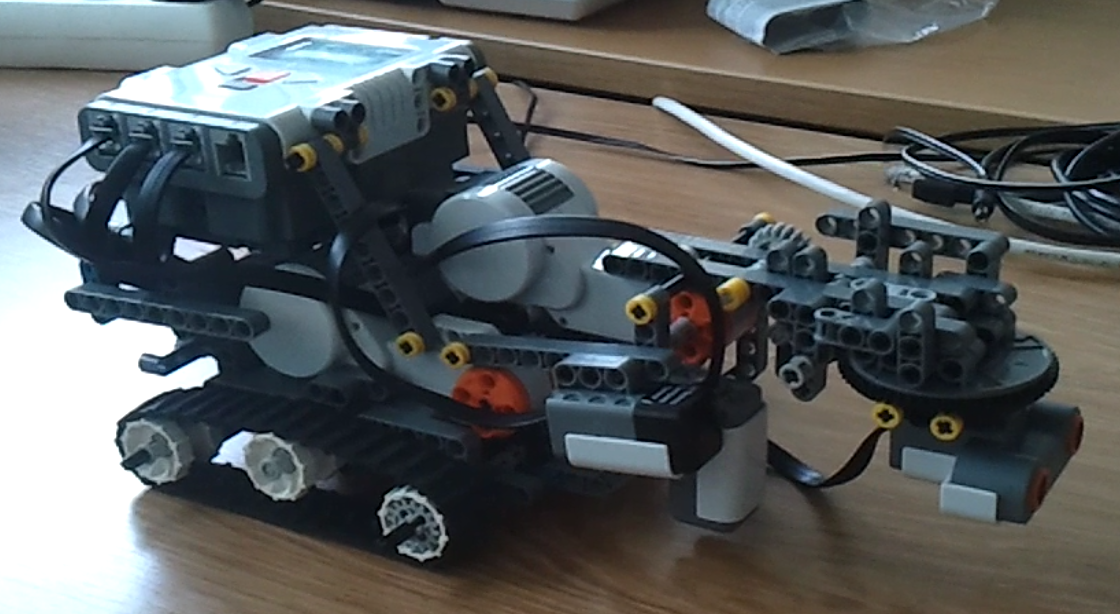
\includegraphics[width=0.9\textwidth, angle=0]{modell1.png}
	\caption{Modell 1}
	\label{modell1}
\end{figure}
\subsubsection{Test}
Getestet haben wir sowohl das Fahrverhalten des Kettenfahrzeuges als auch die Möglichkeit mit dem Radar die Umgebung wahrzunehmen. Hierbei wurde besonders Wert darauf gelegt die Abweichung zum Ist-Wert zu ermitteln.\\
Beim Fahrzeug war es wichtig herauszufinden ob es geradeaus fahren kann und ja mit welcher Abweichung auf verschieden Distanzen (20cm, 50cm, 1m) zu rechnen war. Des Weiteren musste ermittelt werden ob das Fahrzeug in der Lage war sich auf der Stelle zu drehen und dies möglichst genau nach der Vorgabe eines vorher angegeben Winkels. Hierfür wurden mehrere Test mit verschiedensten Winkeln durchgeführt bei denen das Fahrzeug sich so oft drehen musste bis es wieder auf seine Ausgangsposition angelangt ist z.B. vier mal eine Drehung um 90° im Uhrzeigersinn.
Der Radar wurde auf seine Genauigkeit getestet, als auch auf sein Verhalten bei verschiedenen Materialien und Winkel zu den verschiedenen Objekten.
\subsubsection{Pros \& Cons}
Pros:
\begin{itemize}
\item geringe Abweichung bei der Fahrt durch die hohe Reibung der Gummiketten
\item hohe Geländetauglichkeit durch Kettenantrieb
\item kennt das Gebiet vor sich und kann vorausschauend fahren
\end{itemize}
Cons:
\begin{itemize}
\item hohe Abweichung beim drehen
\item sehr hohe Abweichung des Ultraschallsensors wenn nicht im 90° zum Hindernis
\item hohe Ungenauigkeit beim drehen des Radarkopfes durch das Getriebe
\end{itemize}
\subsubsection{Fazit}
Die Idee ist alles in allem nicht schlecht aber die Umsetzung mittels LEGO$^\copyright$ ist nicht praktikabel. Die hohen Ungenauigkeiten und die komplett Aussetzer des Ultraschallsensors lassen uns keine andere Wahl als ein neues Fahrzeug zu entwerfen. Hierbei muss sowohl der Antrieb als auch die Sensorkonstruktion überdacht werden. An einen Einsatz dieses Modells ist nicht zu denken.
\subsection{Idee 2 $\rightarrow$ Modell 2}%angepasstes Grundmodell + riesiger Stoßdämpfer
\subsubsection{Idee}
Da wir bei unserer ersten Idee feststellen mussten das ein kettengetriebenes Fahrzeug zu hohe Ungenauigkeiten verursachte, musste hier eine Alternative gefunden werden, welche aber keine Einschränkungen bei der Bewegungsfreiheit des Fahrzeuges macht d.h. möglichst genaues (vorwärts/rückwärts) Fahren und auf der Stelle wenden können.\\
Auch eine Alternative für den Radar musste her. Hierbei wurde in Kooperation mit dem MCC-Team vereinbart das nicht Hindernisse gefunden werden, sondern davon ausgegangen wird das die gefahren Strecke des Explores frei ist, sozusagen wurde das Bild der Karte invertiert. Dies ermöglichte uns nur auf Hindernisse reagieren zu müssen und nicht wie vorher Informationen über den Bereiche des Einsatzgebietes zu sammeln.
\subsubsection{Konstruktion}
Unsere Konstruktion 2 (siehe Abbildung \ref{modell2} auf Seite \pageref{modell2}) erhielt nun ein 2-Achsen Antrieb, welcher es uns ermöglichte durch gleichzeitiges ansteuern der Motoren gerade Strecken zu fahren, als auch durch entgegengesetztes ansteuern sich auf der Stelle zu drehen. Als Zusatz wurde noch ein Omni-Wheel verbaut, welches dem Gefährt mehr Stabilität verleihen sollte. Um auf Hindernisse reagieren zu können, wurden an der Vorderseite des Fahrzeuges drei Touchsensoren befestigt. Diese sollten auslösen sobald das Fahrzeug vor ein Hindernis fuhr.\\
Verbaute Sensoren und Motoren:
\begin{itemize}
\item zwei Motoren für den Antrieb
\item drei Touch-Sensoren um Hindernisse zu finden
\item ein Lichtstärke-Sensor zur Zielfindung
\end{itemize}
\begin{figure}[ht]
	\centering
  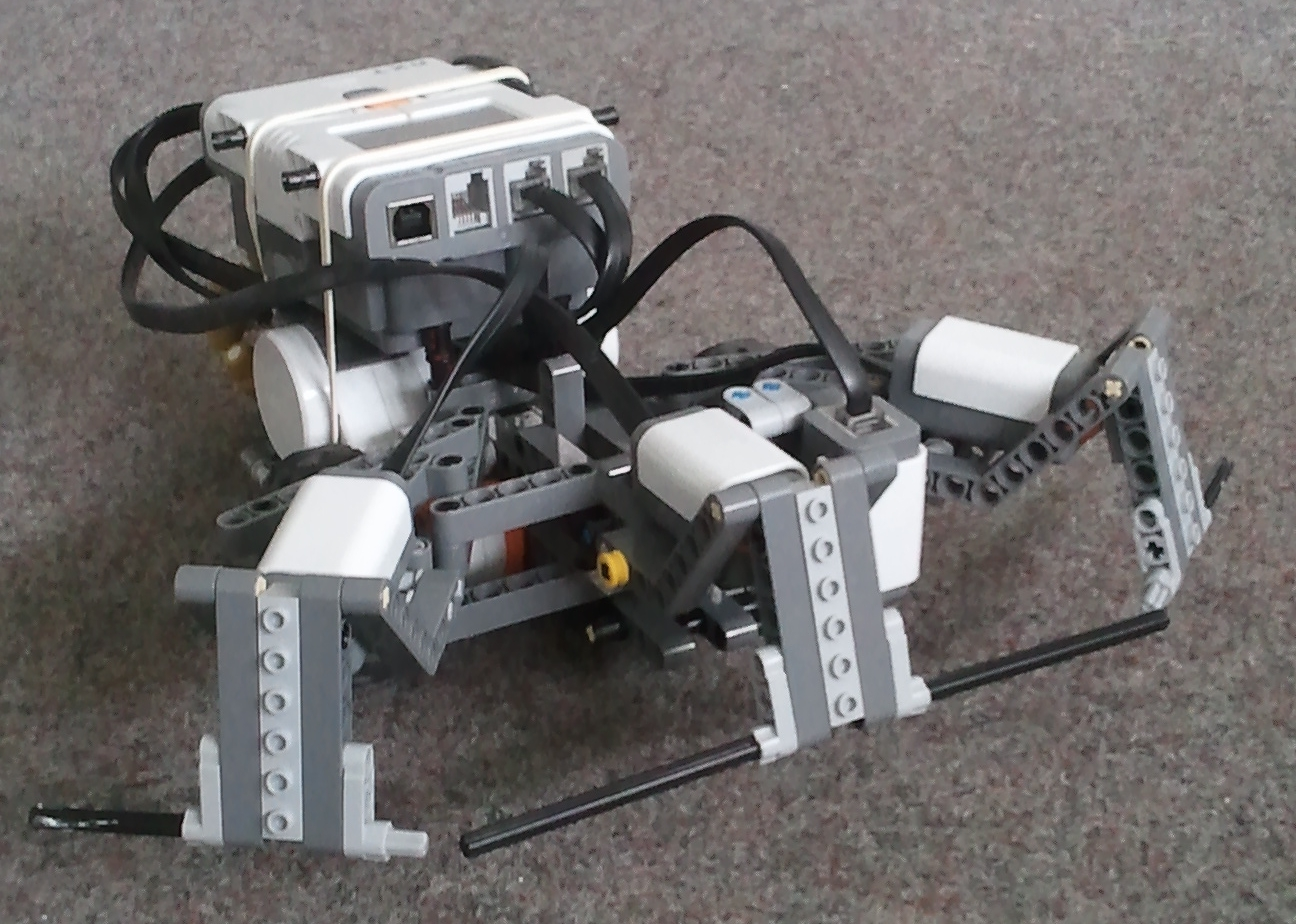
\includegraphics[width=0.9\textwidth, angle=0]{modell2.jpg}
	\caption{Modell 2}
	\label{modell2}
\end{figure}
\subsubsection{Test}
Auch beim zweiten Model wurden die oben schon beschrieben Tests für den Antrieb durchgeführt. Die Sensoren wurden in ihrer Anordnung getestet um eine möglichst optimale Anordnung zu finden. 
\subsubsection{Pros \& Cons}
Pros:
\begin{itemize}
\item geringe Abweichung beim fahren
\item geringe Abweichung beim drehen
\item hohe Aussagekraft bzgl. Sensorevents da nur Touch-Sensoren verbaut wurden
\end{itemize}
Cons:
\begin{itemize}
\item keine Aussagen über das Gebiet vor dem Fahrzeug möglich
\item Fahrzeug kann nur noch reagieren und kaum intelligent handeln
\item Verhaken der Touch-Sensorkonstruktion
\end{itemize}
\subsubsection{Fazit}
Bei der zweiten Konstruktion überzeugt das Antriebsmodel durch seine geringen Abweichungen und seine Agilität. Die Sensoranordnung hingegen lässt noch einige Wünsche offen. Die fehlende Voraussicht ist dabei das größte Manko. An einen Einsatz dieses Model ist ebenfalls nicht zu denken. Eine Verbesserung des Sensorkonstrukts ist nötig.
\subsection{Idee 3 $\rightarrow$ Modell 3}%angepasstes Grundmodell + verbesserte Stoßdämpfer
\subsubsection{Idee}
Das in Idee 2 entwickelte Antriebsmodel hat uns überzeugt. Im dritten Anlauf wird sollte nur noch die Sensoranordnung überdacht werden. Dem Bereich vor dem Fahrzeug sollte dabei mehr Beachtung geschenkt werden, um bessere und intelligentere Entscheidungen treffen zu können.
\subsubsection{Konstruktion}
Bei der dritten Konstruktion (siehe Abbildung \ref{modell3} auf Seite \pageref{modell3}) wurde das Antriebsmodel der zweiten Konstruktion übernommen. Bei den Sensoren wurde der mittlere Touch-Sensor durch ein Ultraschall-Sensor ersetzt. Dieser ermöglichte es die freie Strecke vor dem Fahrzeug zu ermitteln.\\
Verbaute Sensoren und Motoren:
\begin{itemize}
\item zwei Motoren für den Antrieb
\item zwei Touch-Sensoren um Hindernisse zu finden
\item ein Ultraschall-Sensor um den Bereich vor dem Fahrzeug zu überblicken.
\item ein Lichtstärke-Sensor zur Zielfindung
\end{itemize}
\begin{figure}[ht]
	\centering
  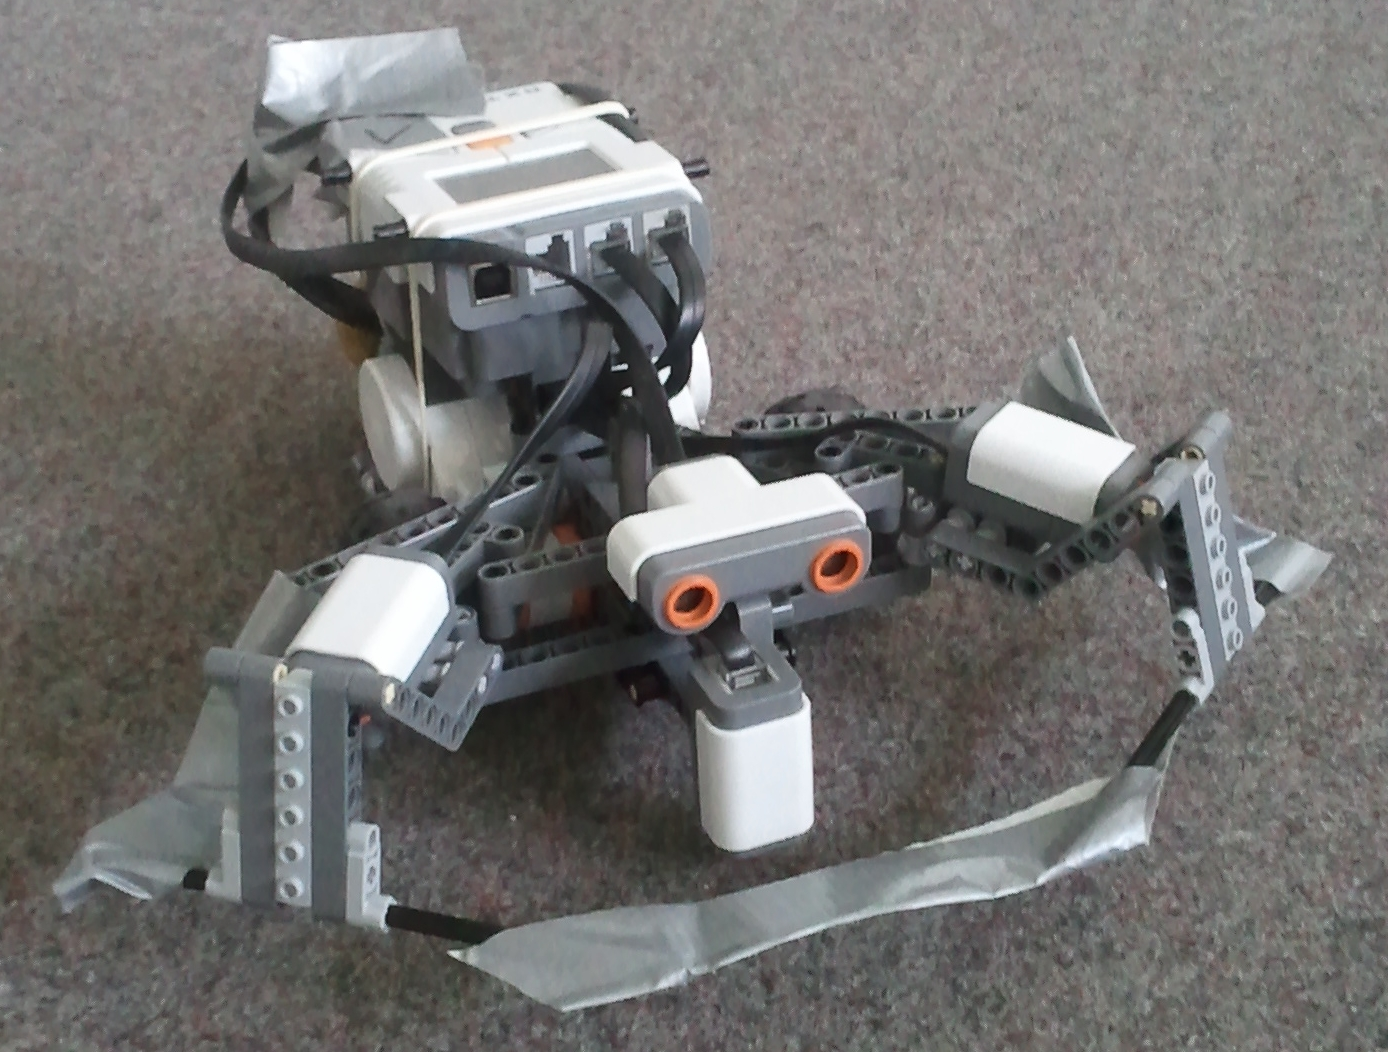
\includegraphics[width=0.9\textwidth, angle=0]{modell3.jpg}
	\caption{Modell 3}
	\label{modell3}
\end{figure}
\subsubsection{Test}
Auch beim dritten Model wurden alle Antriebstests durchgeführt. Die neue Sensoranordnung wurde mit mehreren Testaufbauten auf ihre Einsatztauglichkeit geprüft. Hierbei wurden mögliche Anordnungen von Hindernissen konstruiert und die Sensorevents ausgewertet.
\subsubsection{Pros \& Cons}
Pros:
\begin{itemize}
\item geringe Abweichung beim fahren
\item geringe Abweichung beim drehen
\item freie Strecke vorm Fahrzeug bekannt
\end{itemize}
Cons:
\begin{itemize}
\item Verhaken der Touch-Sensorkonstruktion
\end{itemize}
\subsubsection{Fazit}
Das dritte Model überzeugt durch seinen Antriebsmodel, sowie durch die verbesserte Sensoranordnung gegenüber des zweiten Models. Aber auch dieses Model ist mit Vorsicht zu benutzen. Die Möglichkeiten des Verhaken der Fahrzeuge ist ein großes Problem das es noch zu beseitigen gibt. An einen Einsatz ist nur bedingt zu denken.
\subsection{Fazit und Entscheidung}
Das erste Model ist für raues Gelände bestens geeignet. Durch seine hohen Abweichungen beim Fahren und des nicht zuverlässigen Ultraschall-Sensors im Radar aber kein Kandidat für die Lösung unseres Problems.\\
Das zweite Model überzeugt durch seine Genauigkeit beim Fahren und auch die Aussagekraft der Sensoranordnung. Allerdings fehlt uns hier das gewisse etwas um ein möglichst elegante Lösung für die autonome Erkundung eines Gebietes.\\
Von allen Model schneidet das dritte am besten ab. Es erbt die guten Fahrteigenschaften des zweiten Models und biete uns dazu noch die Möglichkeit durch seine überarbeitete Sensoranordnung möglichst intelligent das Problem zu lösen. 
\section{Kommunikation}
\subsection{Bluetooth}
Bluetooth ist ein Funkstandard speziell für die Nahbereichskommunikation. Er wurde in den 1990er-Jahren von der Bluetooth Special Interest Group (SIG) entwickelt und in IEEE 802.15.1 festgeschrieben. Grundsätzlich sind verbindunglose und verbindungsorientierte Übertragungen möglich. 

Bei der Konzeptionierung von LEGO$^\copyright$ Mindstorms$^\copyright$ NXT hat LEGO$^\copyright$ die Verbindungorientierung für ihre Geräte festgelegt. 
\subsection{Kommunikationsprotokoll PC $\leftrightarrow$ NXT}
Bei einem der Treffen im Rahmen des Semesterprojektes wurde durch den begleitenden Professor  angeregt, dass durch das Team NXT sicherzustellen sei, dass alle Steuerkommandos und Antworten (über Bluetooth) auch von der Gegenstelle erhalten werden müssen. Als Denkanstoß verwies er auf den 3-way-handshake des TCP. Dieser Aspekt wurde von uns mit dem Protokoll aus Abbildung \ref{protokoll_alt} implementiert, sodass auf jede Nachricht vom Typ "`m"' eine Antwort vom Typ "`r"' folgte und der Sende diese Typ "`r"' Nachricht mit einer abschließenden Typ "`a"' Nachricht quittierte. Dieses Protokoll hatte eine Datenflut zur Folge, die kaum zu beherrschen war, da bei überschreiten von Fristen Nachrichten wiederholt gesandt werden mussten. 

Da bei LEGO$^\copyright$ NXT Bluetooth verbindungsorientiert verwendet wird, war die oben beschriebene Herangehensweise nicht nötig, da bei Verbindungsorientiertheit die Zustellung von Nachrichten garantiert wird. Aus diesem Grund wurde das Protokoll auf das in Abbildung \ref{protokoll} reduziert.

Definitions- und Wertebereich der im jüngsten Protokoll (Abbildung \ref{protokoll}) verwendeten Platzhalter:\\
\\
Kommunikation PC $\rightarrow$ NXT:\\
\begin{tabular}{|l|l|p{133mm}|}
\hline \textbf{F} & \textbf{W} & \textbf{Beschreibung} \\ 
\hline 0 & beliebig & Stopp, der NXT in Hardware bricht alle seine Aktionen ab und wartet auf weitere Kommandos\\ 
\hline 1 & 0 -- MAX\_INT & Vorwärtsfahren: bei W = 0 bis Steuerkommando 0 oder Auslösen eines Sensors, bei W~$>$~0 vorwärts fahren für W Grad in Motorumdrehungen\\ 
\hline 2 & 1 -- MAX\_INT & rückwärts fahren für W Grad in Motorumdrehungen  \\ 
\hline 3 & 1 -- MAX\_INT & Fahrzeugachse um W Grad nach links drehen \\ 
\hline 4 & 1 -- MAX\_INT & Fahrzeugachse um W Grad nach rechts drehen \\ 
\hline 5 & beliebig & Messung mit dem Ultraschallsensor ausführen \\ 
\hline 
\end{tabular} \\
\\
\\
Kommunikation PC $\leftarrow$ NXT:\\
\begin{tabular}{|l|l|p{133mm}|}
\hline \textbf{T} & \textbf{W} & \textbf{Beschreibung} \\ 
\hline 1 & 0 -- MAX\_INT & ständige Standortmeldung: für W cm vorwärts gefahren (ohne Kollision)\\
\hline 2 & 1 -- MAX\_INT & Kollision: W cm vorwärts gefahren, Sensor $W_2$ hat ausgelöst\\ 
\hline 3 & 1 -- MAX\_INT & Fahrziel erreicht: für W cm vorwärts gefahren (ohne Kollision) \\ 
\hline 4 & beliebig & Drehung/Rückwärtsfahren beendet \\ 
\hline 5 & 0 -- 255  & Ergebnis der Messung mit dem Ultraschallsensor \\ 
\hline 9 & beliebig & Bodensensor hat Ziel gefunden \\ 
\hline 
\end{tabular} \\
\\
\begin{figure}[h]
Kommunikation PC $\rightarrow$ NXT:$\qquad$
\begin{bytefield}[bitwidth=2em]{7}
\bitheader{0-6} \\
\bitbox{1}{A} & \bitbox{1}{;} & \bitbox{1}{ID} & \bitbox{1}{;} & \bitbox{1}{F} & \bitbox{1}{,} & \bitbox{1}{W}
\end{bytefield}\\
~\\
Kommunikation PC $\leftarrow$ NXT:$\qquad$
\begin{bytefield}[bitwidth=2em]{9}
\bitheader{0-8} \\
\bitbox{1}{A} & \bitbox{1}{;} & \bitbox{1}{ID} & \bitbox{1}{;} & \bitbox{1}{T} & \bitbox{1}{,} & \bitbox{1}{W} & \bitbox{1}{,$_2$} & \bitbox{1}{W$_2$}
\end{bytefield}
\\
\\
\texttt{\underline{Legende:}\\ A = Typ der Nachricht (m = Nachricht, r = m erhalten, a = r erhalten)\\ F = Funktion die aufgerufen werden soll\\ W = Zahlwert \\ T = Typ der Antwort\\ $_2$ = optional}
\caption{Kommunikationsprotokoll 3-way-handshake}\label{protokoll_alt}
\end{figure}
\begin{figure}[h]
Kommunikation PC $\rightarrow$ NXT:$\qquad$
\begin{bytefield}[bitwidth=2em]{5}
\bitheader{0-4} \\
\bitbox{1}{ID} & \bitbox{1}{;} & \bitbox{1}{F} & \bitbox{1}{,} & \bitbox{1}{W}
\end{bytefield}\\
~\\
Kommunikation PC $\leftarrow$ NXT:$\qquad$
\begin{bytefield}[bitwidth=2em]{7}
\bitheader{0-6} \\
\bitbox{1}{ID} & \bitbox{1}{;} & \bitbox{1}{T} & \bitbox{1}{,} & \bitbox{1}{W} & \bitbox{1}{,$_2$} & \bitbox{1}{W$_2$}
\end{bytefield}
\\
\\
\texttt{\underline{Legende:}\\ F = Funktion die aufgerufen werden soll\\ W = Zahlwert \\ T = Typ der Antwort\\ $_2$ = optional}

\caption{Kommunikationsprotokoll}\label{protokoll}
\end{figure}
\subsection{Kommunikation mit dem MCC}
Für die Kommunikation mit dem MCC kam das Python Framework Twisted\footnote{http://twistedmatrix.com} zum Einsatz. Twisted ist ein sogenanntes "`event-driven"' framework, das heißt der Programmierer stellt für Aktionen Callback-Funktionen bereit. Twisted abstrahiert von der darunterliegenden Netzwerkarchitektur und dem verfügbaren Netzwerkprotokollstack (wenn auch nicht vollständig transparent), dies vereinfacht die Programmierung eines Verteilten Systems erheblich.
\section{Logik}
Für die logische Programmierung des "`Explorers"' bestand vorwiegend das Problem, dass die Hardware (der Brick) Zeit benötigt um die Aktionen auszuführen, also blockiert, jedoch die Softwarekomponente asynchrones Messaging nutzt. Um diese Hürde zu überwinden wurde bei der Konzeptionierung des Systems darauf geachtet, dass auf jedes Steuerkommando, welches eine Handlung der Hardware hervorruft, nach Abschluss der Handlung eine Antwort des Brick gesendet werden muss. Dass versetzte uns in die Lage mit einer synchronisierten boole'schen Variablen (blockiert = True) die Software solange zu blockieren, bis die Antwort vom Brick eingegangen ist und damit die boole'sche Variable wieder auf False gesetzt wird.
\subsection{Explorationsalgorithmen}
In der Welt der autonomen Rasenmäh- und Staubsaugroboter haben sich vier Algorithmen durchgesetzt\footnote{Quelle: Roboter mit Mikrocontrollern, Heinz Schmid, Franzis Verlag, 2011}:
\begin{enumerate}
\item Touch and Go\footnote{hier simple genannt} 
\item circle
\item radar
\item Wandverfolgung
\end{enumerate}
1 -- 3 werden im Folgenden näher besprochen. 4 konnte aufgrund der begrenzten Anzahl an Sensoren nicht implementiert werden und bleibt deshalb außen vor. 
\subsubsection{Exploration -- simple}
Der erste und auch gleichzeitig einfachste Algorithmus. Der Roboter fährt solange geradeaus bis er auf ein Hindernis trifft. Nach dem Auslösen eines Sensors wechselt der Roboter beliebig seine Fahrtrichtung und fährt wieder geradeaus bis zum nächsten Ereignis. Der Explorer wechselt die Richtung nicht vollständig beliebig, er wählt die Drehrichtung in Abhängigkeit von dem auslösenden Sensor, soll heißen wenn der linke Sensor angeschlagen wurde, dreht sich der Explorer um einen beliebigen Winkel zwischen 30° und 160° nach rechts.
\subsubsection{Exploration -- circle}
Wie in Abbildung \ref{circle} zu sehen ist macht der Explorer eine Bewegungsabfolge in Form einer eckigen Nautilusschnecke. Durch diese Bewegungsfolge wird der Bereich in dem sich der Explorer befindet schnell erkundet.

In Abbildung \ref{state_circle} wird an Hand eines Zustandsautomaten gezeigt, wie der Explorationsalgorithmus umgesetzt ist. Es gibt keinen ausgezeichneten Endzustand, was damit begründet ist, dass der Algorithmus von einem externen Zähler abgebrochen wird. Der Abbruch kann in jedem der Zustände geschehen. Man kann erkennen, dass zusätzlich zur reinen Bewegung weitere Zustände und Transitionen eingefügt wurden um Messungen mit dem Ultraschallsensor durchzuführen. Die Messungen dienen als Grundlage zur Berechnung eines Korrekturfaktors für alle Bewegungen.
\begin{figure}[h]
\centering
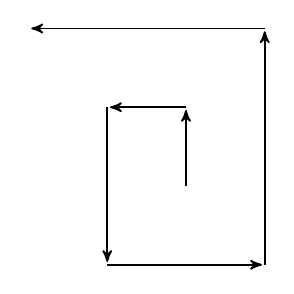
\begin{tikzpicture}[->,>=stealth',shorten >=1pt,auto,node distance=2.8cm,
                    semithick]
  \tikzstyle{every state}=[fill=red,draw=none,text=white]

  \coordinate  (A) at (0,0);
  \coordinate  (B) at (0,1);
  \coordinate  (C) at (-1,1);
  \coordinate  (D) at (-1,-1);
  \coordinate  (E) at (1,-1);
  \coordinate  (F) at (1,2);
  \coordinate  (G) at (-2,2);

  \path (A) edge (B)
        (B) edge (C)
        (C) edge (D)
        (D) edge (E)
        (E) edge (F)
        (F) edge (G);

\end{tikzpicture}
\caption{Bewegungsmuster Exploration -- circle}
\label{circle}
\end{figure}
\begin{figure}[h]
\centering
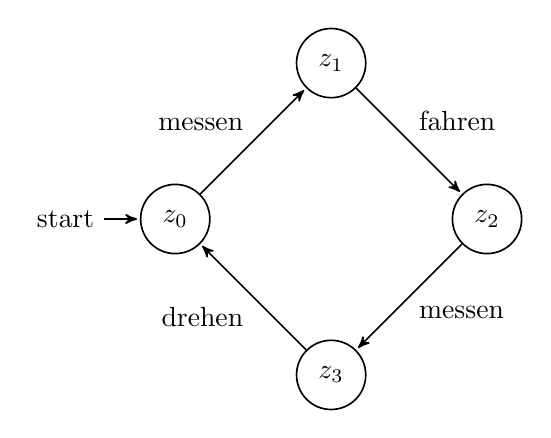
\begin{tikzpicture}[->,>=stealth',shorten >=1pt,auto,node distance=2.8cm,
                    semithick]
  \tikzstyle{every state}=[draw,text=black]

  \node[initial,state] (z0)                     {$z_0$};
  \node[state]         (z1) [above right of=z0] {$z_1$};
  \node[state]         (z2) [below right of=z1] {$z_2$};
  \node[state]         (z3) [below right of=z0] {$z_3$};


  \path (z0) edge node {messen} (z1)
        (z1) edge node {fahren} (z2)
        (z2) edge node {messen} (z3)
        (z3) edge node {drehen} (z0);

\end{tikzpicture}
\caption{state-machine Exploration -- circle}
\label{state_circle}
\end{figure}
\subsubsection{Exploration -- radar}
Wie in Abbildung \ref{radar} zu sehen ist, macht der Explorer eine Bewegungsabfolge in Form einer eckigen Wellenausbreitung. Durch diese Bewegungsfolge wird der Bereich vor dem Explorer schnell erkundet und der Explorer verlässt langsam seinen bisherigen Bereich.

Wie im Abschnitt Exploration -- circle wird hier auch ein Zustandsautomat (Abbildung \ref{state_radar}) zur Darstellung des Algorithmus verwendet. Er unterliegt den gleichen Kriterien wie oben.
\begin{figure}[h]
\centering
\begin{tikzpicture}[->,>=stealth',shorten >=1pt,auto,node distance=2.8cm,
                    semithick]
  \tikzstyle{every state}=[fill=red,draw=none,text=white]

  \coordinate  (A) at (0,0);
  \coordinate  (B) at (0,1);
  \coordinate  (C) at (2,1);
  \coordinate  (D) at (2,2);
  \coordinate  (E) at (-3,2);
  \coordinate  (F) at (-3,3);
  \coordinate  (G) at (5,3);

  \path (A) edge (B)
        (B) edge (C)
        (C) edge (D)
        (D) edge (E)
        (E) edge (F)
        (F) edge (G);

\end{tikzpicture}
\caption{Bewegungsmuster Exploration -- radar}
\label{radar}
\end{figure}
\begin{figure}[h]
\centering
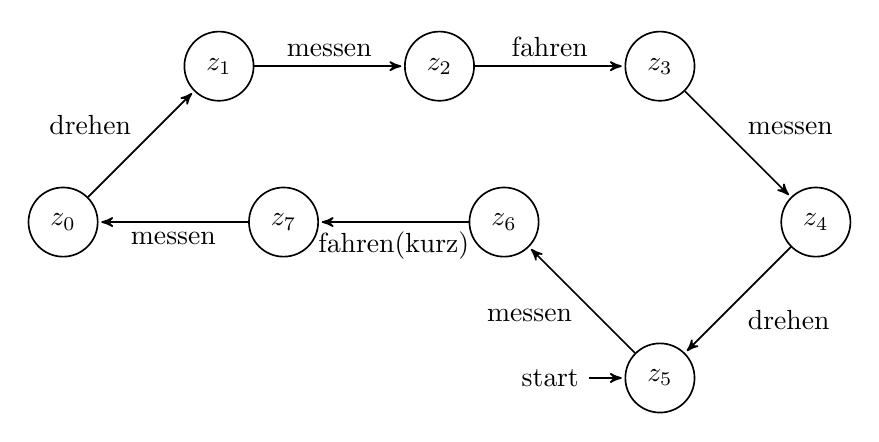
\begin{tikzpicture}[->,>=stealth',shorten >=1pt,auto,node distance=2.8cm,
                    semithick]
  \tikzstyle{every state}=[draw,text=black]

  \node[state] 		   (z0)                     {$z_0$};
  \node[state]         (z1) [above right of=z0] {$z_1$};
  \node[state]         (z2) [right of=z1] {$z_2$};
  \node[state]         (z3) [right of=z2] {$z_3$};
  \node[state]         (z4) [below right of=z3] {$z_4$};
  \node[initial,state]         (z5) [below left of=z4] {$z_5$};
  \node[state]         (z6) [above left of=z5] {$z_6$};
  \node[state]         (z7) [left of=z6] {$z_7$};


  \path (z0) edge node {drehen} (z1)
        (z1) edge node {messen} (z2)
        (z2) edge node {fahren} (z3)
        (z3) edge node {messen} (z4)
        (z4) edge node {drehen} (z5)
        (z5) edge node {messen} (z6)
        (z6) edge node {fahren(kurz)} (z7)
        (z7) edge node {messen} (z0);

\end{tikzpicture}
\caption{state-machine Exploration -- radar}
\label{state_radar}
\end{figure}
\subsection{GoToPoint}
Für die GoToPoint -- Funktionalität wurden die zwei Funktionen aus Listing \ref{listing1} und Listing \ref{listing2} benötigt. Mit der Funktion berechnePunkt() kann aus der eigenen Ausrichtung, der gefahrenen Entfernung und dem ehemaligen Standort der neu Standort berechnet werden. Die Funktion berechneVektor() aus Listing \ref{listing2} berechnet zu zwei gegebenen Punkten den verbindenden Vektor, dazu wird erst ein relatives Koordinatensystem geschaffen, dann wird über den Satz von Pythagoras die Entfernung, d.h. der Betrag des Vektor berechnet und danach Winkel berechnet.
\begin{figure}[h]
\begin{lstlisting}[language={python}, caption={berechnePunkt()}\label{listing1},captionpos=t]
def berechnePunkt(ausrichtung, entfernung, standort = {'x':0.0, 'y':0.0}):
    return {'x': standort['x'] + entfernung * GRAD2CM * 
    			 math.cos(ausrichtung * (math.pi / 180.0)),
            'y': standort['y'] + entfernung * GRAD2CM * 
            	 math.sin(ausrichtung * (math.pi / 180.0))}
\end{lstlisting}
\end{figure}
\begin{figure}[h]
\begin{lstlisting}[language={python}, caption={berechneVektor()}\label{listing2},captionpos=t]
def berechneVektor(standort = {'x':0.0, 'y':0.0}, ziel = {'x': 0.0, 'y': 0.0}):
    relativ_ziel = {'x': abs(ziel['x'] - standort['x']), 
    				'y': abs(ziel['y'] - standort['y'])}
    dbg_print("StO: (%d,%d), Z: (%d,%d), rZ: (%d,%d)"%(standort['x'],
                                                       standort['y'],
                                                       ziel['x'], 
                                                       ziel['y'], 
                                                       relativ_ziel['x'], 
                                                       relativ_ziel['y']), 1, 0)
    entfernung = math.sqrt(relativ_ziel['x'] ** 2 + relativ_ziel['y'] ** 2)
    if relativ_ziel['x'] == 0:
        winkel = 90
    elif relativ_ziel['x'] < 0:
        winkel = math.atan(float(relativ_ziel['y']) / float(relativ_ziel['x'])) * 
        		 (180.0 / math.pi) + 180
    else:
        winkel = math.atan(float(relativ_ziel['y']) / float(relativ_ziel['x'])) * 
        		 (180.0 / math.pi) + 360
    return {'winkel': winkel % 360, 
    		'entfernung': entfernung, 
    		'rel_x': relativ_ziel['x'], 
    		'rel_y': relativ_ziel['y']}
\end{lstlisting}
\end{figure}
\end{document}
